\chapter{General Introduction}
\label{chap:general-introduction}

\section{Motivation and Context}
\label{sec:general-motivation}

Data-driven research increasingly depends on access to detailed datasets, yet the same level of detail that makes data useful can also make it sensitive. In areas such as healthcare, finance, public administration, and social science, individual-level records often cannot be shared freely because of legal, ethical, and institutional constraints. Synthetic data has therefore become an important candidate for privacy-preserving analysis: instead of releasing the original records, a generator produces artificial observations intended to preserve the statistical properties needed for research \cite{rubin1993, little1993, nowok2016}.

The practical value of synthetic data, however, cannot be judged only by whether the generated records look plausible. The central question is whether an analyst using the synthetic data would reach conclusions similar to those obtained from the original data. This is the problem of analytical utility. Prior work distinguishes between broad similarity measures and task-specific utility measures, emphasizing that the right evaluation depends on the downstream analysis being supported \cite{snoke2018}.

This thesis studies synthetic-data utility from that downstream perspective. It asks whether common synthesis methods preserve enough information for two different families of machine-learning and statistical analysis:
\begin{itemize}
  \item \textbf{clustering}, where the relevant utility is structural and geometric;
  \item \textbf{regression}, where the relevant utility is inferential and concerns coefficients, uncertainty, and confidence intervals.
\end{itemize}

\section{Machine-Learning Perspective}
\label{sec:general-ml-perspective}

Machine learning includes a broad set of methods that learn from data rather than relying on explicitly programmed rules. A common taxonomy distinguishes between supervised learning, unsupervised learning, and reinforcement learning. Figure~\ref{fig:ml_taxonomy} summarizes this classification and positions the two analytical settings studied in this thesis.

\begin{figure}[H]
  \centering
  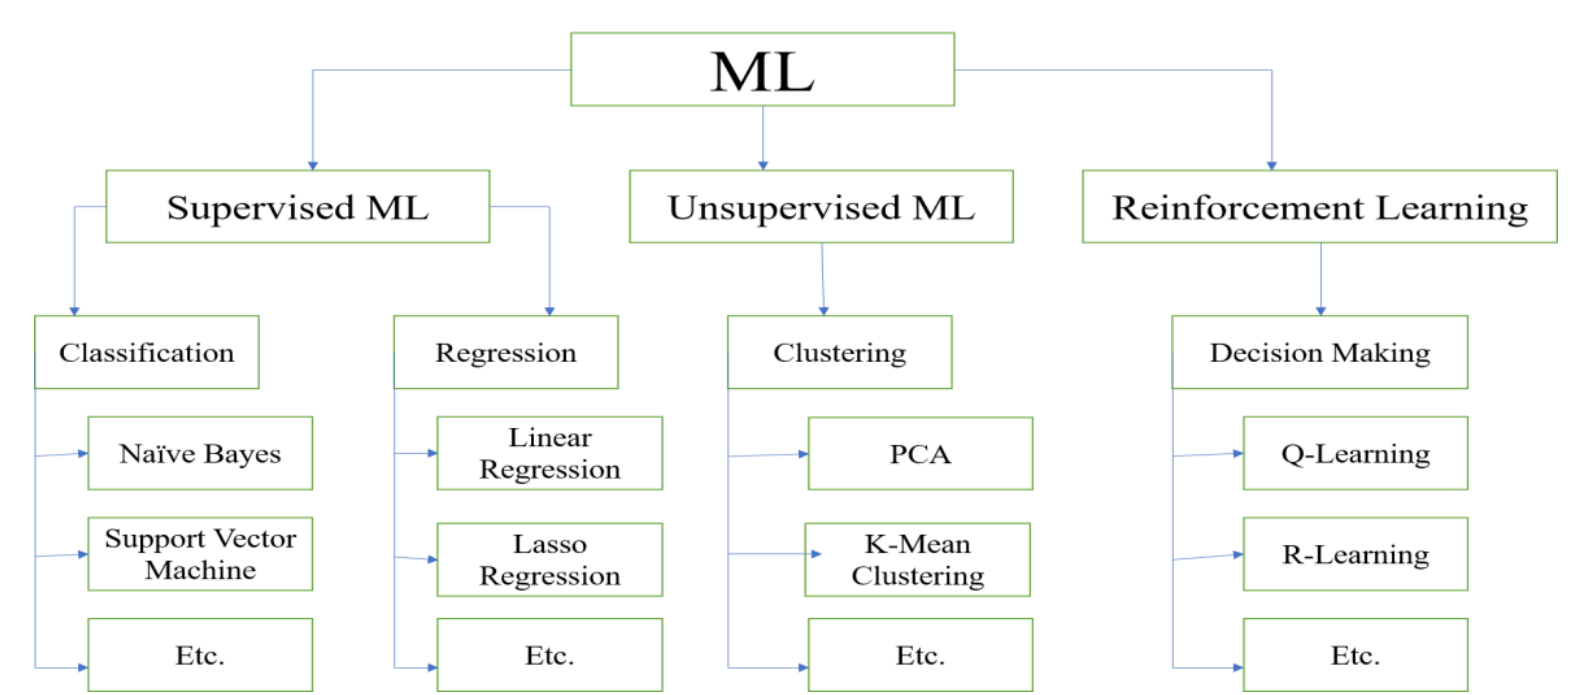
\includegraphics[width=0.85\linewidth]{figures/parts/01_Introduction/01_General_Introduction/ML_types.png}
  \caption[Taxonomy of machine-learning paradigms]{Taxonomy of common machine-learning paradigms and representative algorithms.}
  \label{fig:ml_taxonomy}
  \source{Compiled by the author}
\end{figure}

Regression belongs to the supervised or model-based inferential setting, because it studies how an outcome changes as a function of predictors. Clustering belongs to unsupervised learning, because it attempts to discover structure without observing ground-truth labels during training. These two settings place different demands on synthetic data, as summarized in Table~\ref{tab:utility-types}.

\begin{table}[H]
  \centering
  \caption[Comparison of Structural and Inferential Utility]{Comparison of Structural and Inferential Utility demands on synthetic data.}
  \label{tab:utility-types}
  \renewcommand{\arraystretch}{1.3}
  \begin{tabular}{@{}lp{5cm}p{5cm}@{}}
    \toprule
    \textbf{Dimension} & \textbf{Structural Utility (Clustering)} & \textbf{Inferential Utility (Regression)} \\ \midrule
    \textbf{Learning Paradigm} & Unsupervised & Supervised / Model-based \\
    \textbf{Primary Goal} & Preserve geometry and separability & Preserve relationships and uncertainty \\
    \textbf{Key Features} & Distances, densities, topology & Point estimates, standard errors, CIs \\
    \textbf{Sensitivity} & High sensitivity to spatial artifacts & High sensitivity to correlation limits \\
    \bottomrule
  \end{tabular}
  \source{Compiled by the author based on \cite{reiter2003, drechsler2011}}
\end{table}

Clustering requires preservation of distances, densities, separability, and cluster geometry. Regression requires preservation of conditional relationships, point estimates, standard errors, and confidence intervals \cite{reiter2003, drechsler2011}.

\section{Formal Problem Definition}
\label{sec:general-problem}

The motivating assumption behind synthetic data is that a generated dataset can act as a useful substitute for the original data. However, the practical value of this substitution depends heavily on the ``Privacy vs. Utility'' trade-off. To generalize the problem and evaluate this trade-off rigorously, we must treat both clustering and regression as algorithms that extract a specific set of parameters or structural truths from a given dataset. By formalizing this extraction process, we can quantify the exact degradation introduced by synthesis.

\subsection{The Core Unified Framework}
We define the fundamental spaces and operators involved in the analytical lifecycle:

\begin{itemize}
    \item \textbf{The Original Data:} Let $\mathcal{D}_{R}$ be the real (reference) dataset of size $N$ drawn from a true underlying joint probability distribution $P(X, Y)$ \cite{nowok2016}. For unsupervised clustering tasks, $Y = \emptyset$, and the analysis focuses solely on the feature space $X$.
    \item \textbf{The Synthetic Generator:} Let $\mathcal{G}$ be a synthetic generation mechanism, such as the CART method which models variables via sequential conditional distributions. We define the resulting synthetic dataset as:
    \begin{equation}
        \mathcal{D}_{S} = \mathcal{G}(\mathcal{D}_{R})
    \end{equation}
    \item \textbf{The Learning Algorithm:} Let $\mathcal{A}$ represent a machine learning algorithm applied to a dataset to extract a vector of learned properties or parameters, $\theta$.
    \begin{itemize}
        \item \textit{In Clustering:} $\mathcal{A}$ represents algorithms like K-Means or Hierarchical Clustering. The extracted parameters $\theta$ represent geometric structures, such as the number of clusters $k$, centroids $\mu$, and within-cluster variance $\sigma^{2}$.
        \item \textit{In Regression:} $\mathcal{A}$ represents supervised models like Linear or Logistic regression. Here, $\theta$ represents inferential relationships, primarily the estimated coefficients $\hat{\beta}$ and their associated standard errors or confidence intervals.
    \end{itemize}
\end{itemize}

\subsection{The Generalized Utility Discrepancy}
The fundamental problem addressed in this thesis is evaluating the \textbf{Utility Discrepancy} caused by the generation mechanism $\mathcal{G}$. We aim to quantify the degradation between the true parameters learned from the real data, $\theta_{R} = \mathcal{A}(\mathcal{D}_{R})$, and the parameters learned from the synthetic proxy, $\theta_{S} = \mathcal{A}(\mathcal{D}_{S})$.

We define a task-specific discrepancy function $\Delta(\theta_{R}, \theta_{S})$ that measures the loss of structural or inferential fidelity. The core research problem is to evaluate how $\Delta$ is influenced by the data space complexity, which is bounded by:
\begin{equation}
    \Delta(\mathcal{A}(\mathcal{D}_{R}), \mathcal{A}(\mathcal{G}(\mathcal{D}_{R}))) = f(N, p, \rho, S)
\end{equation}
Where the degradation is parameterized as a function of:
\begin{itemize}
    \item $N$: The sample size of the dataset.
    \item $p$: The dimensionality (number of variables or predictors).
    \item $\rho$: The correlation structure or degree of cluster separation.
    \item $S$: The distributional shape or skewness (e.g., Normal vs. Gamma distributions).
\end{itemize}

\subsection{Task-Specific Instantiations of the Discrepancy Function \texorpdfstring{($\Delta$)}{(Delta)}}
To apply this generalized framework to the specific studies in the thesis, we instantiate $\Delta$ using the metrics tailored for each domain. These instantiations serve as the mathematical foundation for evaluating both unsupervised and supervised downstream tasks.

\textbf{A. The Clustering Instantiation (Geometric Fidelity)}

For unsupervised learning, the discrepancy function $\Delta$ measures topological and spatial distortion. The target parameters $\theta$ are the centroid locations ($\mu$) and the internal cluster variance. This thesis formalizes the discrepancy via the Mean Centroid Distance (MCD) and Mean Variance Difference (MVD). The MCD instantiation is defined as:
\begin{equation}
    \Delta_{\text{MCD}}(\theta_{R}, \theta_{S}) = \frac{1}{k}\sum_{j=1}^{k}||\mu_{j}^{(R)}-\mu_{j}^{(S)}||_{2}
\end{equation}
The analytical goal is to prove that for non-parametric generators like CART applied to skewed data ($S = \text{Gamma}$), $\Delta_{\text{MCD}}$ diverges significantly when the algorithm $\mathcal{A}$ requires convex/spherical assumptions (such as K-Means) compared to connectivity-based methods (such as Hierarchical Clustering).

\textbf{B. The Regression Instantiation (Inferential Fidelity)}

For supervised learning, $\Delta$ measures the distortion of conditional probabilities and statistical uncertainty. The target parameters $\theta$ are the point estimates ($\hat{\beta}$) and their Confidence Intervals ($[L, U]$). The discrepancy is formalized using the Bias Ratio ($B_{R}$) and Confidence Interval Overlap (CIO). To frame CIO as a penalty or discrepancy that should be minimized, we utilize $1 - \text{CIO}$:
\begin{equation}
    \Delta_{\text{Inference}}(\theta_{R}, \theta_{S}) = 1 - \frac{1}{2}\left(\frac{\min(U_{R},U_{S})-\max(L_{R},L_{S})}{U_{R}-L_{R}} + \frac{\min(U_{R},U_{S})-\max(L_{R},L_{S})}{U_{S}-L_{S}}\right)
\end{equation}
The analytical goal here is to demonstrate that sequentially compounding errors in the generator $\mathcal{G}$ over high dimensions ($p$) and high multicollinearity ($\rho$) artificially scales the variance of $\theta_{S}$, causing the inferential discrepancy to increase, particularly in small-sample logistic settings.

\section{Objectives and Research Questions}
\label{sec:general-objectives}

The general objective of this thesis is to evaluate whether synthetic data preserves downstream analytical utility across two complementary settings: clustering and regression.

The specific objectives are:
\begin{enumerate}
  \item To evaluate whether CART-generated synthetic data preserves the geometric structure required by clustering algorithms.
  \item To compare the robustness of centroid-based and connectivity-based clustering under synthetic distortions.
  \item To evaluate whether synthetic data preserves regression coefficients and confidence intervals in linear and logistic models.
  \item To compare CART-based synthesis with parametric synthesis when the downstream analysis has a known model structure.
  \item To identify conditions under which synthetic data remains useful, becomes unstable, or leads to misleading analytical conclusions.
\end{enumerate}

These objectives are addressed through three thesis-level research questions:
\begin{itemize}
  \item \textbf{RQ1:} Does synthetic data preserve the structural geometry required for unsupervised clustering?
  \item \textbf{RQ2:} Does synthetic data preserve the inferential quantities required for regression analysis?
  \item \textbf{RQ3:} How does the match between generator assumptions, data structure, and downstream analytical method determine synthetic-data utility?
\end{itemize}

\section{Structure of the Thesis}
\label{sec:general-structure}

The thesis is divided into two empirical studies under this common framing.

\textbf{Part I} studies structural utility for clustering. It evaluates K-Means and Agglomerative Hierarchical Clustering on CART-generated synthetic datasets, using controlled simulations and structural metrics such as cluster-number recovery, Gini coefficient, Mean Centroid Distance, and Mean Variance Difference.

\textbf{Part II} studies inferential utility for regression. It evaluates linear and logistic regression under CART and parametric synthesis, using Confidence Interval Overlap, Bias Ratio, and Confidence Interval Width Ratio to measure whether synthetic data supports the same statistical conclusions as the original data.

The final discussion integrates both studies and presents the overall thesis conclusion: synthetic data should be selected and validated according to the analysis it is expected to support, not treated as a universally interchangeable replacement for original data.
